\begin{frame}[c]{Aufgabenbereiche}
	\begin{columns}[c]
		\begin{column}{0.2\textwidth}
			\begin{tikzpicture}
				\draw circle (1) [path picture={ 
						\node at (path picture bounding box.center){
						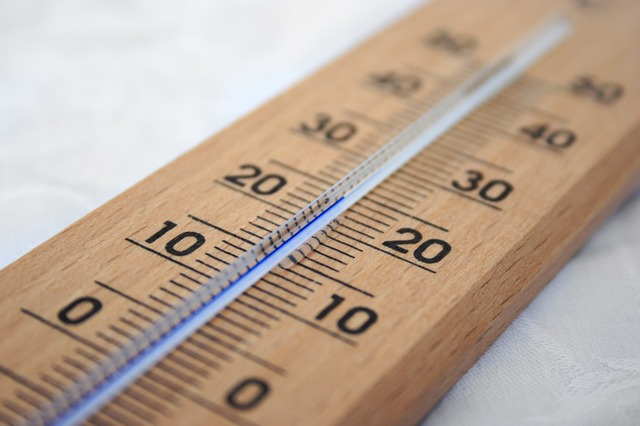
\includegraphics[height=2cm]{picture/thermometer.jpg}};}, 
						line width=1];
				\end{tikzpicture}
			\end{column}
			\begin{column}{0.8\textwidth}
				\begin{block}{Datennahme}
					Temperatur, Luftfeuchtigkeit, Druck, Wolkendecke und
					abgeleitete Größen	
				\end{block}
			\end{column}
		\end{columns}

		\vspace{0.2cm}	
		\begin{columns}[c]
			\begin{column}{0.2\textwidth}
				\begin{tikzpicture}
					\draw circle (1) [path picture={ 
							\node at (path picture bounding box.center){
							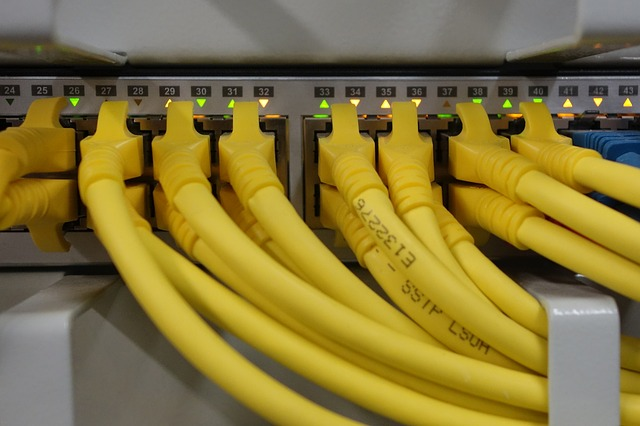
\includegraphics[height=2cm]{picture/network.jpg}};}, 
							line width=1];
					\end{tikzpicture}
				\end{column}
				\begin{column}{0.8\textwidth}
					\begin{block}{Transfer}
						Vom Einplatinencomputer zum Server
					\end{block}
				\end{column}
			\end{columns}

			\vspace{0.2cm}	
			\begin{columns}[c]
				\begin{column}{0.2\textwidth}
					\begin{tikzpicture}
						\draw circle (1) [path picture={ 
								\node at (path picture bounding box.center){
								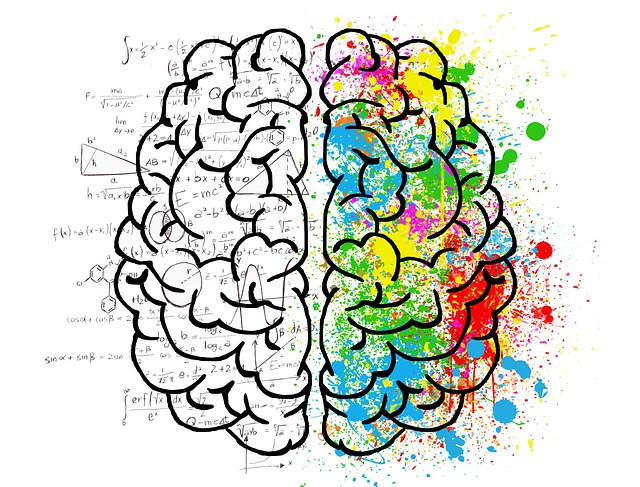
\includegraphics[height=2cm]{picture/brain.jpg}};}, 
								line width=1];
						\end{tikzpicture}
					\end{column}
					\begin{column}{0.8\textwidth}
						\begin{block}{Analyse}
							Wettervorhersagen und Wolkenklassifizierung
						\end{block}
					\end{column}
				\end{columns}

			\end{frame}
